\chapter{Реализация и экспериментальная проверка}
\label{chapter4}

В этой главе описывается, как была реализована система пошаговой бета-редукции и её синтаксические анализаторы на платформе .NET/F\#. Приведены ключевые фрагменты кода, описаны инструменты, структура ПО, сценарии работы, тестовые примеры и сравнительный анализ с существующими решениями.

\section{Выбор инструментальных средств}
Для реализации использовались:
\begin{itemize}
  \item Платформа \textbf{.NET 8.0+} и язык \textbf{F\#} — за выразительность в работе с AST и рекурсивными типами.
  \item Библиотека \textbf{FParsec} для построения парсера в комбинаторном стиле.
  \item NUnit для модульного тестирования.
  \item Visual Studio / Rider для разработки и отладки.
\end{itemize}

\section{Состав и структура реализованного ПО}
\label{sec:software-structure}

Результат работы оформлен как набор модулей F\#, упакованных в единый NuGet‑пакет \texttt{Mephi.Cybernetics.Mace.BetaReduction}. Реализованное ПО является библиотекой классов на языках C\# и F\# на платформе .NET 8.0+. Основные компоненты:

\begin{itemize}
  \item \texttt{BetaReduction.Parser}  
    \begin{itemize}
      \item Построен на библиотеке FParsec.  
      \item Содержит класс \texttt{BRParser} (реализует \texttt{ILanguageParser}):  
        \begin{itemize}
          \item Конфигурация через \texttt{Config}, где задаются списки унарных и бинарных операторов, ключевые слова и флаги.
          \item Колбэки \texttt{pVariableCallback}, \texttt{pNumericCallback}, \texttt{pKeywordCallback} для превращения токенов в объекты \texttt{ITerm}.
          \item Исключения \texttt{BRParsingException} для унифицированной обработки ошибок разбора.
        \end{itemize}
      \item Парсер легко расширяется: достаточно добавить в \texttt{Config.operators} новый \texttt{UnOp} или \texttt{BinOp}, либо расширить список \texttt{keywords}.
    \end{itemize}

  \item \texttt{BetaReduction.Machine}  
    \begin{itemize}
      \item Содержит абстрактную машину \texttt{BetaReductor} (реализует \texttt{IAbstractMachine}):  
        \begin{itemize}
          \item \texttt{CreateDefaultState}, \texttt{EvaluateCode} и \texttt{EvaluateState} для пошагового и полного редуцирования.
          \item Типы-обёртки \texttt{Code(term: ITerm)} и \texttt{State(code, stepNum, isFinal)} для хранения текущего терма, номера шага и флага завершённости.
          \item Рекурсивная функция \texttt{evaluateOneStep} обрабатывает бета‑редексы, атомарные вызовы (\texttt{IAtomic.ReduceWithArguments}) и погружение в тело абстракций.
          \item Полная нормализация реализована как рекурсивный цикл вызовов \\\texttt{evaluateOneStep}.
        \end{itemize}
      \item Регистрами машины выступает единственный регистр \texttt{Term}, что упрощает визуализацию каждого шага.
    \end{itemize}

  \item \texttt{BetaReduction.Environment \& Atomic}  
    \begin{itemize}
      \item \texttt{Environment} — коллекция \texttt{ITff} и \texttt{IAtomic}, настраиваемая в зависимости от домена (BR vs CAM).  
      \item \texttt{Atomic} — набор предопределённых атомиков (\texttt{Int}, \texttt{Bool}, арифметические и логические операторы, \texttt{IfComb}, \texttt{YComb}).  
      \item Каждый атомик реализует интерфейс \texttt{IAtomic}:  
        \texttt{Arity}, \texttt{IsReducibleWith} и \texttt{ReduceWithArguments} описывают семантику.
    \end{itemize}


\noindent
Каждый из перечисленных модулей структурирован по принципу «один файл — одна ответственность», что упрощает поддержку и развитие проекта. Весь исходный код легко интегрируется в другие .NET‑проекты и может быть опубликован как NuGet‑пакет.


\section{Основные сценарии работы}
\begin{enumerate}
  \item \textbf{Разбор выражения:} 
    \[
      \texttt{let term = BRParser().Parse("\textbackslash x -> x x")}
    \]
    — возвращает AST (\texttt{ITerm}).
  \item \textbf{Пошаговая редукция:} 
    \[
      \texttt{let state = BetaReductor(cfg).EvaluateCode(code, true)}
    \]
    — один шаг.
  \item \textbf{Полная нормализация:} 
    \[
      \texttt{BetaReductor(cfg).EvaluateCode(code, false)}
    \]
    — до нормальной формы.
\end{enumerate}

\section{Ключевые фрагменты кода}

\subsection{Настройка парсера}
Комбинаторный подход на FParsec: конфигурация операторов и колбэков вынесена в отдельный блок, что упрощает расширение:

\begin{lstlisting}[
  float=tb,frame=lines,
  label=lst:parser-config,
  caption=Конфигурация BRParser: операторы, ключевые слова и колбэки
]
// определить унарные и бинарные операторы с приоритетами
let brUnOps = [ UnOp {| keyword = "-"; term = atomicUnOpMinus; priority = 1 |} ]
let brBinOps = [
  BinOp {| keyword = "+"; term = atomicBinOpPlus;   priority = 1; 
        associativity = Associativity.Left |}
  BinOp {| keyword = "*"; term = atomicBinOpMult;   priority = 2; 
        associativity = Associativity.Left |}
  // ...
]

// объединить в конфиг
let cfg = {
  applicationTff     = appTff
  simpleLambdaTff    = SimpleLambdaTff(subs)
  multiLambdaTff     = Some (MultiLambdaTff(subs))
  operators          = brUnOps @ brBinOps
  keywords           = ["true"; "false"; "Y"; "NULL"]
  parseNumericConsts = true
  ifStatements       = false
}

// привязать колбэки для переменных, чисел, ключевых слов
p.pVariableCallback <- fun name -> DefaultVariable(name) :> ITerm
p.pNumericCallback  <- fun n    -> match n with Int i -> Data.Int i | 
    Float f -> Data.Float f
p.pKeywordCallback  <- function
  | "true"  -> Data.Bool true
  | "false" -> Data.Bool false
  | kw      -> raise (BRParsingException ...)
\end{lstlisting}

Пример задания конфигурации BRParser представлен в листинге \ref{lst:parser-config}.

\subsection{Механизм одного шага редукции}
Внутри \texttt{BetaReductor} ключевая функция \texttt{step} обрабатывает:
\begin{itemize}
  \item \textbf{β-редексы:} $(\lambda x.M)\,N \to M[x:=N]$;
  \item \textbf{спуск внутрь:} если редексов нет, рекурсивно обходит подтермы;
  \item \textbf{атомарные функции:} вызывает \texttt{IFunction.ReduceWithArguments}.
\end{itemize}

\begin{lstlisting}[
  float=tb,frame=lines,
  label=lst:machine-step,
  caption=Алгоритм одного шага в BetaReductor
]
let rec step term =
  match term with
  | :? IApplicationTerm as app ->
      match app.Function with
      | :? SimpleLambda as lam ->
          // бета-редукция: подстановка первого аргумента
          let arg = Seq.head app.Arguments
          substitution.Substitute(lam.Body, seq { lam.Variable, arg })
      | f when f :? IFunction ->
          // атомарный вызов
          f.ReduceWithArguments(app.Arguments, tff)
      | _ ->
          // спуск внутрь
          // 1) пытаемся step(f)
          // 2) если не изменилось, пробуем step на каждом аргументе
          term
  | :? IFunctionalAbstraction as lam ->
      // спуск внутрь тела λ
      let body' = step lam.GetBody
      if not (obj.ReferenceEquals(body', lam.GetBody)) then
        // пересоздать лямбду с новым телом
        SimpleLambda(lam.GetBoundVariable, body', substitution) :> ITerm
      else term
  | _ -> term
\end{lstlisting}

Алгоритм шага редукции представлен в листинге \ref{lst:machine-step}.

\section{Разработка тестовых примеров}
\label{sec:test-examples}

Для обеспечения надёжности и корректности работы как парсера, так и абстрактной машины бета‑редукции, был разработан обширный набор NUnit‑тестов.

\subsection{Тесты парсера}

Нижеследующие аспекты разбора покрываются тестами из модуля \texttt{ParseTest}:

\begin{itemize}
  \item \textbf{Лямбда‑абстракции:} проверяется, что строка вида \verb|\ x -> x| корректно преобразуется в \texttt{SimpleLambda}.  
  \item \textbf{Унарные и бинарные операторы:} приоритеты и ассоциативность обрабатываются в соответствии с конфигурацией \texttt{unOps} и \texttt{binOps}.  
  \\
  \item \textbf{Вложенные абстракции и приложения:} тестируются случаи \(\lambda x.\,\lambda y.\,\lambda z.\,y\) и \((\lambda x.\,x+x)\,5\).  
  \item \textbf{Скобочные конструкции:} проверяется различие между \(\,x + x - x\) и \(\,x + (x - x)\).  
  \item \textbf{Ключевые слова:} пользовательские ключевики (\texttt{magicWord0}, \texttt{magicWord1}) обрабатываются через колбэк \texttt{pKeywordCallback}.  
\end{itemize}

\begin{lstlisting}[float=tb,frame=lines,label=lst:parser-test-example,caption={Пример теста для скобочных выражений}]
[<Test>]
member this.Parentheses() =
  let noPar = "\\ x -> x plus x - x"
  let withPar = "\\ x -> x plus (x - x)"
  let gotNo = callParse2String(parser, noPar)
  let gotPar = callParse2String(parser, withPar)
  Assert.That(gotNo, Is.EqualTo(expectedNo))
  Assert.That(gotPar, Is.EqualTo(expectedPar))
\end{lstlisting}

Пример теста для скобочных выражений представлен в листинге \ref{lst:parser-test-example}.

\subsection{Тесты бета‑редуктора}

Тестовый модуль \texttt{BetaReductionTests} проверяет корректность шаговой и полной редукции:

\begin{itemize}
  \item \textbf{Один шаг vs. полная нормализация:} для терма \((\lambda x.\,x\,x)\,x\) сравнивается результат одного шага и финальной формы.  
  \item \textbf{Последовательность шагов:} функция \texttt{reduceStepByStep} строит весь путь редукции, и каждый промежуточный результат сравнивается с ожидаемым списком строковых представлений термов.  
  \item \textbf{Атомарные операции:} проверка встроенных бинарных операций, например \((+\,1\,2)\to 3\).  
  \item \textbf{Композиция λ‑выражений:} тесты для вложенных абстракций, например \(((\lambda x.\,x)\,(\lambda x.\,x))\) приводят к корректному результату.  
\end{itemize}

\begin{lstlisting}[float=tb,frame=lines,label=lst:reductor-step-test,caption={Проверка последовательности шагов редукции}]
[<Test>]
member _.``step by step plus``() =
  let plus = Data.BinOp("+", fun a b -> match a,b with Int x,Int y -> 
        Int(x+y) | _ -> failwith "")
  let term = applicationTff.CreateTerm([ plus; Data.Int 1; Data.Int 2 ])
  let seq = reduceStepByStep reductor (term2Code term)
  Assert.That(seq |> List.last, Is.EqualTo("Int 3"))
\end{lstlisting}

Проверка последовательности шагов редукции представлена в листинге \ref{lst:reductor-step-test}.

\section{Сравнение с существующими аналогами}
\label{sec:comparison-analogs}

Было произведени сравнение разработанным в данной работе решением с одним из аналогов визуализации работы абстррактной машины \textbf{WinCam} (см. рис.~\ref{fig:wincam}).


\subsection*{Преимущества WinCam}
\begin{itemize}
  \item Имеется визуализация термов в представлении де Брейна.
  \item Разработана встроенная справочная книга с набором готовых учебных примеров.
  \item Поддерживается выбор учебного языка из фиксированного набора.
\end{itemize}

\subsection*{Недостатки WinCam}
\begin{itemize}
  \item Интерфейс устаревший, перегруженный и плохо адаптирован под начинающих пользователей.
  \item Отсутствует модульность — невозможно добавить собственные вычислительные стратегии, лексемы или атомики без изменения исходного кода.
  \item Программа работает только под Windows и основана на устаревшем .NET Framework, что делает её недоступной для пользователей Linux и macOS.
\end{itemize}

\subsection*{Преимущества разработанного решения}
\begin{itemize}
  \item Реализована архитектура, ориентированная на расширяемость: пользователи могут определять собственные атомики (\texttt{IAtomic}), языковые конструкции (\texttt{ILanguageParser}) и стратегии редукции.
  \item Предусмотрена возможность свободного переключения между абстрактными машинами.
  \item Приложение сопровождается справочником с примерами, документацией и шаблонами использования.
  \item Кроссплатформенность — работает на Windows, Linux и macOS благодаря использованию .NET 8.0+.
\end{itemize}

\begin{figure}[h]
  \centering
  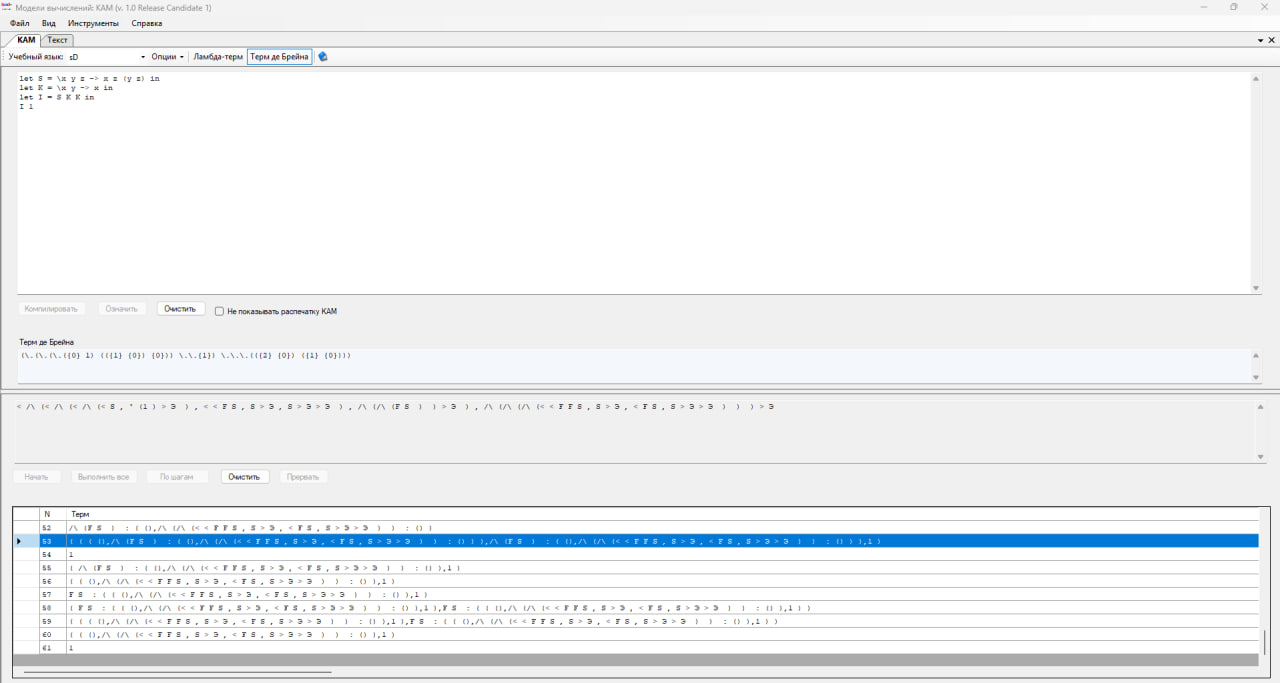
\includegraphics[width=0.8\textwidth]{./img/WinCam.png}
  \caption{Интерфейс WinCam: лямбда‑терм, отображение терма де Брейна и шаги КАМ}
  \label{fig:wincam}
\end{figure}

Графический пользовательский интерфейс WinCam представлен на рис. \ref{fig:wincam}.



\section{Выводы}
\begin{itemize}
  \item В данной главе была представлена реализация бета-редуктора на платформе .NET с использованием языка F\# и библиотеки FParsec. Основное внимание было уделено структуре программного обеспечения, принципам модульности и расширяемости, ключевым компонентам (парсер, абстрактная машина, атомики) и механизмам настройки.
  \item Были разработаны сценарии использования системы — от разбора выражения до полной нормализации — и подтверждена корректность их реализации с помощью модульных тестов на базе NUnit. Предложенные подходы к конфигурации синтаксического анализатора и построению редуктора позволяют эффективно адаптировать систему под различные домены и языки.
  \item Сравнение с системой WinCam, показало, что разработанное решение обладает более современной архитектурой, кроссплатформенностью и гибкостью. Оно предоставляет пользователю расширенные возможности по настройке языка, визуализации и интеграции в другие проекты .NET.
\end{itemize}
Таким образом, реализованная система представляет собой современный, расширяемый и тестируемый инструмент для пошаговой редукции λ-термов, пригодный как для образовательных, так и для исследовательских целей.
